%%%%%%%%%%%%%%%%%%%%%%%
% Theoretical Background
%%%%%%%%%%%%%%%%%%%%%%%%

\chapter{Theoretical Background}\label{chap:2}

\section{Overview}
Rayleigh-B\'{e}nard-Poiseuille (RBP) flows describe the motion of fluids confined between two infinitely extended parallel walls, heated from below and cooled from the top, driven by a pressure gradient.
\begin{figure}[h]
\centering
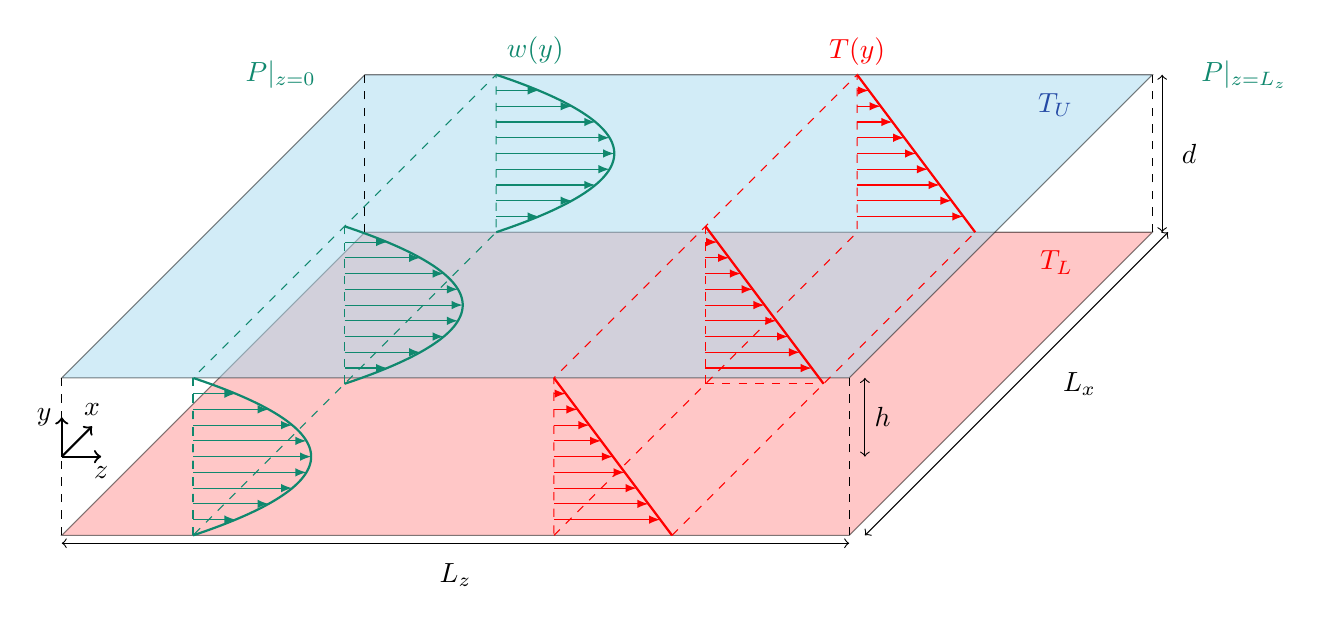
\begin{tikzpicture}
\def\H{1}
\def\W{10}
\def\L{10}

% Draw the bottom plate
\draw [fill=pink!75!red, opacity=0.5] (-\L/2,-\H,0) -- (\L/2,-\H,0) -- (\L/2, -\H, -\W) -- (-\L/2, -\H,-\W) -- cycle;

% Draw the top plate
\draw [fill=SkyBlue!75!white, opacity=0.5] (-\L/2,\H,0) -- (\L/2,\H,0) -- (\L/2, \H, -\W) -- (-\L/2,\H,-\W) -- cycle;

%  % Draw axes
\draw [dashed, thin] (-\L/2, -\H, 0) -- (-\L/2, \H, 0);
\draw [dashed, thin] (\L/2, -\H, 0) -- (\L/2, \H, 0);
\draw [dashed, thin] (\L/2, -\H, -\W) -- (\L/2, \H, -\W);
\draw [dashed, thin] (-\L/2, -\H, -\W) -- (-\L/2, \H, -\W);
%\draw [dashed, thin] (-1,0, 0) --++ (\L,0,0) --++ (0,0,-\W) --++ (-\L,0,0) -- cycle;
%  % \draw [thin, dashed] (-1,0) -- (6,0);

% Add dimensions
% L_x
\draw [<->] (-\L/2,-1.1*\H, 0) -- (\L/2,-1.1*\H,0);
\node[centered] at (0,-1.5*\H,0) {$L_z$};
 
% L_z
\draw [<->] (\L/2*1.025, -\H, -\W) -- (\L/2*1.025, \H,-\W);
\node[right] at (\L/2*1.05,0.0,-\W) {$d$};

% d
\draw [<->] (\L/2*1.04, -\H) -- (\L/2*1.04,-\H,-\W);
\node[centered] at (\L/2*1.2,-\H,-\W/2) {$L_x$};

% h
\draw [<->] (\L/2*1.04, 0, 0) -- (\L/2*1.04, \H, 0);
\node[right] at (\L/2*1.04,\H/2,0) {$h$};

% P
\node[left] at (-\L/2*1.1, \H, -\W) {\textcolor{PineGreen}{$P|_{z=0}$}};
\node[right] at (\L/2*1.1, \H, -\W) {\textcolor{PineGreen}{$P|_{z=L_z}$}};

% T
\node[left] at (\L/2*0.9, \H, -\W*0.9) {\textcolor{cyan!20!blue}{$T_U$}};
\node[left] at (\L/2*0.9, -\H, -\W*0.9) {\textcolor{red}{$T_L$}};

% Draw labels
\draw[->, thick] (-\L/2, 0, 0) -- (-\L/2,\H/2,0) node[left] {$y$};
\draw[->, thick] (-\L/2, 0, 0) -- (-\L/2+\H/2,0,0) node [below] {$z$};
\draw[->, thick] (-\L/2, 0, 0) -- (-\L/2,0,-\H) node[above] {$x$};

% Draw the velocity profile
\draw[PineGreen,thick,domain=-1:1,samples=200,smooth] plot ({(1-\x*\x)*1.5-\L/3}, \x) node[above right] {};
\draw[PineGreen,thick,domain=-1:1,samples=200,smooth] plot ({(1-\x*\x)*1.5-\L/3}, \x, -\W/2) node[above right] {};
\draw[PineGreen,thick,domain=-1:1,samples=200,smooth] plot ({(1-\x*\x)*1.5-\L/3}, \x, -\W) node[above right] {$w(y)$};
\draw[-,PineGreen,dashed] (-\L/3,-\H) -- (-\L/3,\H);
\draw[-,PineGreen,dashed] (-\L/3,-\H, -\W/2) -- (-\L/3,\H, -\W/2);
\draw[-,PineGreen,dashed] (-\L/3,-\H,0) -- (-\L/3,\H,0) -- (-\L/3,\H,-\W) -- (-\L/3,-\H,-\W) -- cycle;

\foreach \y in {-0.8,-0.6,...,0.8} {
    \draw[-latex,PineGreen] (-\L/3,\y, 0) -- ({(1-\y*\y)*1.5-\L/3},\y,0);
    \draw[-latex,PineGreen] (-\L/3,\y, -\W/2) -- ({(1-\y*\y)*1.5-\L/3},\y, -\W/2);
    \draw[-latex,PineGreen] (-\L/3,\y, -\W) -- ({(1-\y*\y)*1.5-\L/3},\y,-\W);
}

% Draw the temperature profile
\draw[red,thick,domain=-\H:\H,samples=200,smooth] plot ({(1/2*(1-\x)*1.5+\L/8)}, \x);
\draw[red,thick,domain=-\H:\H,samples=200,smooth] plot ({(1/2*(1-\x)*1.5+\L/8)}, \x, -\W/2);
\draw[red,thick,domain=-\H:\H,samples=200,smooth] plot ({(1/2*(1-\x)*1.5+\L/8)}, \x, -\W);
\draw[-,red,dashed] (\L/8,-\H,-\W/2) -- (\L/8,\H,-\W/2);
\draw[-,red,dashed] (\L/8,-\H,-\W/2) -- (\L/8 + 1.5,-\H,-\W/2);
\draw[-,red,dashed] (\L/8 +1.5,-\H,0) -- (\L/8 + 1.5,-\H,-\W);
\draw[-,red,dashed] (\L/8,-\H,0) -- (\L/8,-\H,-\W) -- (\L/8,\H, -\W) -- (\L/8,\H,0) -- cycle;
% % 
\foreach \y in {-0.8,-0.6,...,0.8} {
   \draw[-latex,red] (\L/8,\y) -- ({\L/8+(1/2*(1-\y)*1.5},\y);
   \draw[-latex,red] (\L/8,\y, -\W/2) -- ({\L/8+(1/2*(1-\y)*1.5},\y, -\W/2);
   \draw[-latex,red] (\L/8,\y, -\W) -- ({\L/8+(1/2*(1-\y)*1.5},\y, -\W);
}
% Add labels
\node[above,red] at (\L/8,1,-\W) {$T(y)$};
\end{tikzpicture}
\label{fig:rbpconfiguration}
\caption{The Rayleigh-B\'{e}nard Poiseuille (RBP) flow configuration.}
\end{figure}

The RBP configuration is illustrated in figure \ref{fig:rbpconfiguration}, where $z^*, y^*, x^*, L_z, L_x, d, h$ refer to the streamwise, spanwise, wall-normal coordinates, length, span, depth and half-height of the domain respectively.
We note that the asterisks$^*$, refer to variables in dimensional form.
The flow is driven by a pressure gradient along the streamwise $z^*$ direction, $\Delta P^* = P^*|_{z^*=0} - P^*|_{z^*=L_z} < 0$, leading to the formation of a laminar Poiseuille flow, $w^*(y^*)$, for a sufficiently small $\Delta P$. 
In this study, we will only consider fully-developed flow, where the boundary layer from the top and the bottom wall meets at the midplane, $y^*=0$, and entrance effects are neglected.
The RBP configuration is also unstably stratified, such that the temperature difference between the lower, $T_L$, and upper wall, $T_U$, is always positive, $\Delta T = T_L - T_U > 0$, leading to a stable linear conduction profile along the wall-normal direction, $T(y^*)$, if $\Delta T$ is kept sufficiently small.

The RBP system combines the two paradigmatic flow configurations; the classical Rayleigh-B\'{e}nard convection (RBC) and the plane Poiseuille flow (PPF), driven by buoyancy and shear forces, respectively.
In the absence of a pressure gradient, the RBP configuration reduces to the classical Rayleigh-B\'{e}nard convection problem, bringing about buoyany-driven convection for a sufficiently large unstable stratification.
In the limiting case without unstable stratification, $\Delta T = 0$, the system reduces to the wall-bounded plane Poiseuille flow (PPF), where the transition towards subscritical shear-driven turbulence may be expected for a sufficiently large pressure gradient.

The onset of convection and the transition to subscritical shear-driven turbulence has been well studied independently over the past decades, however, the transitional regime where both forces interact remains largely unexplored.
For instance, do buoyancy forces promote the transition to shear-driven turbulence and how does shear influence the convection? 
Understanding the transition to turbulence in this regime can have implications for applications such as the fabrication of thin uniform films in chemical vapour deposition \citep{evans_unsteady_1991,jensen_flow_1991,fauzi_critical_2018} and the cooling of electronic components \citep{kennedy_combined_1983,ray_analysis_1992}.
To describe the motion of the fluid in RBP configurations, we cosider non-dimensionalised Navier-Stokes equations with Boussinessq approximations,
\begin{subequations}\label{eq:rbp_equations}
\begin{equation}
    \frac{\partial \mathbf{u}}{\partial t} + (\mathbf{u}\cdot\nabla)\mathbf{u} = -\nabla p + \frac{1}{Re}\nabla^2 \mathbf{u} + \frac{Ra}{Re^2Pr} \theta,
\end{equation}
\begin{equation}
    \frac{\partial \theta}{\partial t} + (\mathbf{u} \cdot \nabla)\theta = \frac{1}{RePr}\nabla^2 \theta,
\end{equation}
\begin{equation}
    \nabla \cdot \mathbf{u} = 0.
\end{equation}
\end{subequations}
where $\mathbf{u}(\mathbf{x}), \theta(\mathbf{x}), p(\mathbf{x})$ refers to the nondimensionalised velocity, temperature and presure respectively.
The key control parameters for RBP flows are the Rayleigh number, $Ra$, Reynolds number, $Re$, Prandlt number $Pr$, which are defined as follows,
\begin{equation}
    Ra = \eta g d^3 \Delta T / \nu \kappa, \quad Re = W_c h / \nu, \quad Pr = \kappa / \nu, \quad \Gamma = L/2d,
\end{equation}
where $\eta, g, \Delta T, \nu, \kappa, W_c, h, d, L$ are the thermal expansion coefficient, acceleration due to gravity, temperature difference between the bottom and top wall, kinematic viscosity, thermal diffusivity, laminar centreline velocity, domain's half-depth, full-depth, length or span respectively.

We first discuss the key developments of plane Poiseuille flow (PPF) outlining the key theoretical framework for analysing the stability of fluid flows. This is then followed by Rayleigh-B\'{e}nard convection (RBC) in \S \ref{sec:bkgrd_RBC}.
The historical developments involving Rayleigh-B\'{e}nard Poiseuille (RBP) flows are then expanded in \S \ref{sec:bkgrd_RBP} concluded by a section describing the hydrodynamic stability of fluid flows in \S \ref{sec:bkgrd_transitional}

%%%%%%%%%%%%%%%%%%%%%%%%
% Plane Poiseuille Flows
%%%%%%%%%%%%%%%%%%%%%%%%

\section{Transitional wall-bounded shear flows}\label{sec:bkgrd_transitional}
Wall-bounded shear flows remain as a fundamental topic in fluid mechanics, concerning the motion of a fluid travelling in parallel to solid surfaces (such as walls), where pressence of the wall influences the flow.
To satistfy the non-slip boundary conditions at the walls, the fluid layer becomes sheared, leading to velocity gradients and shear stresses within the fluid.
The prototypical examples flows include the pressure-driven plane Poiseuille flow (PPF), pipe (Hagen-Poiseuille) flow, plane Couette flow and flat plate boundary layers.
These geometrically simple examples enables a convenient framework amenable to the mathematical analysis of fluid motion under shear.
A central question in this field is predicting the transition to turbulence, specifically, at what point does turbulence emerge as shear increases?
% One of the central questions is on the prediction on the transition to turbulence, specifically, when is turbulence expected as shear is increased?
% plane Poiseuille flow (PPF) describes the motion of a fluid confined between two infinitely extended parallel walls, driven by a pressure gradient, also referred to as channel flow.
% It belongs to a general class of wall-bounded shear flows, consisting of plane Couette flow, pipe (Hagen-Poiseuille) flow and flat plate boundary layer flow.

The earliest investigation into this transition dates back to the pipe flow experiments of \cite{reynolds_xxix_1883}.
In his experimental setup, the flow speed through the pipe could be controlled by regulating the inlet pressure, while injecting dye to visualise the flow, as illustrated in figure \ref{fig:reynolds}(a).
At low speeds, the fluid remained laminar, whereby the fluid layers moved in smooth parallel `laminates', resulting to a single streak of steady dye in figure \ref{fig:reynolds}(b).
As the speed increased, the dye begin to exhibit irregular `sinuous' motions interspersed with laminar regions shown in figure \ref{fig:reynolds}(c).
This is now referred to as the transitional/intermittent regime, alternating between the laminar and turbulent states.
Beyond a critical speed, the dye breaks down entirely into chaotic `eddies', mixing with the surrounding fluid and discolouring the flow with dye downstream in figure \ref{fig:reynolds}(d).
This regime is now identified as turbulence.
Reynolds conjectured that the threshold between the laminar, transitional and turbulent regimes could be characterised by non-dimenisonal parameter, now known as the Reynolds number, $Re = U D/\nu$, where $U$ is the centerline velocity in the pipe, $D$, the pipe diameter and $\nu$, the kinematic viscosity.
He observed that flow through the pipe remained `stable' and laminar for $Re < 1900$, while it became `unstable' and turbulent for $Re > 2000$ \citep{reynolds_iv_1895}.
His remarks led to the concept of the stability of fluid flows.
\begin{figure}[h]
    \centering
    \includegraphics[width=1\textwidth]{Background/Figures/Reynolds.pdf}
    \caption{(a) Osbourne Reynolds pipe experiment with the dye injection apparatus, illustrating the (b) laminar flow, (c) intermittent regime and (d) turbulent flow as the flow speed is increased, taken from \citep{reynolds_xxix_1883}.}
    \label{fig:reynolds}
\end{figure}

%%%%%%%%%%%%%%%%%%%%%%%%%%%
% Linear Stability Analysis
%%%%%%%%%%%%%%%%%%%%%%%%%%%

\subsection{Linear Stability Analysis}
Following Reynolds' experiment, interest towards the mathematical analysis of the stability of fluid flows grew in early $20^{st}$ century.
The typical approach begins with decomposing the velocity field, $\mathbf{u}(\mathbf{x},t)$, into a laminar (base) state, $U(y)$ (assumed to depend only on the wall-normal direction here), and the velocity perturbations, $\mathbf{u}'(\mathbf{x},t)$, with pressure similarly decomposed as,
\begin{equation}
    \mathbf{u}(\mathbf{x}) = U(y) + \mathbf{u}'(\mathbf{x},t), \quad \text{and} \quad p(\mathbf{x},t) = P(x) + p'(\mathbf{x},t).
\end{equation}
Next, we the substitute the formulations for the decomposed velocity and pressure into the Navier-Stokes equations of equation \eqref{eq:rbp_equations} and drop the nonlinear pertubrations terms $(\mathbf{u'}\cdot \nabla)\mathbf{u'}$,
\begin{subequations}\label{eq:shear_linearised}
\begin{equation}
    \frac{\partial \mathbf{u'}}{\partial t} + (U \cdot\nabla)\mathbf{u'} + (\mathbf{u'}\cdot\nabla)U= -\nabla p' + \frac{1}{Re}\nabla^2 \mathbf{u'},
\end{equation}
\begin{equation}
    \nabla \cdot \mathbf{u}' = 0,
\end{equation}
\end{subequations}
resulting to the linearised Navier-Stokes equations. 
This commonly followed by introducing a wavelike ansatz (mode) defined by streamwise and spanwise wavenumbers, $\alpha, \beta$ and complex frequency, $\omega$.
In general two ways to analysis the linearised Navier-Stokes equations by considering the behaviour of each mode independently in \S \ref{subsec:modal} and their coupled dynamics in \S \ref{subsec:nonmodal}

%%%%%%%%%%%%%%%%%
% MODAL STABILITy
%%%%%%%%%%%%%%%%%

\subsubsection{Modal analysis}\label{subsec:modal}
It is covenient to eliminate the pressure terms by to transform equation \eqref{eq:shear_linearised} using the wall-normal perturbation velocity, $v'$, and wall-normal vorticity, $\eta' = \partial u'/ \partial z - \partial w' / \partial x$, variables.
Using $(v, \eta)$, introduce an ansatz (mode) for them,
\begin{equation}\label{eq:shear_ansatz}
    v'(\mathbf{x},t ) = \tilde{v}(y)e^{i(\alpha x + \beta z - \omega t)}, \quad \text{and} \quad \eta'(\mathbf{x}, t) = \tilde{\eta}(y)e^{i(\alpha x + \beta z - \omega t)}.
\end{equation}
where $\alpha, \beta, \omega$ denotes the streamwise and spanwise wavenumbers, and complex frequency (i.e. $\omega = \omega_r + i\omega_i$), respectively.
Next, we substitute the ansatz into equation \ref{eq:shear_linearised}, leading to the classical Orr-Sommerfeld and Squire equations \citep{orr_stability_1907,sommerfeld_beitrag_1909,squire_stability_1933, schmid_stability_2001},
\begin{equation}\label{eq:OSQ}
    \left[
    -i\omega 
    \begin{pmatrix}
        k^2 - \mathcal{D}^2 & 0 \\
        0 & 1 
    \end{pmatrix}
    + 
    \begin{pmatrix}
        \mathcal{L}_{OS} & 0 \\
        i\beta U' & \mathcal{L}_{SQ} 
    \end{pmatrix}
\right ]
    \begin{pmatrix}
        \tilde{v} \\
        \tilde{\eta}
    \end{pmatrix}
    = \mathbf{0},
\end{equation}
where $\mathcal{L}_{OS}$ and $\mathcal{L}_{SQ}$ refers to the Orr-Sommerfeld and Squire operators given as,
\begin{subequations}
  \begin{equation} 
      \mathcal{L}_{OS} = i\alpha U(k^2-\mathcal{D}^2) + i\alpha U'' + \frac{1}{Re}(k^2 - \mathcal{D}^2)^2,
  \end{equation}
  \begin{equation} 
      \mathcal{L}_{SQ} = i\alpha U + \frac{1}{Re}(k^2 - \mathcal{D}^2).
  \end{equation}
\end{subequations}
$k^2, \mathcal{D}, U', U''$ denotes the sum of squared wavenumbers, $k^2 = \alpha^2 + \beta^2$, differential operator in $y$, first- and second- derivative of the laminar velocity, respectively.
Equation \eqref{eq:OSQ} is simply an eigenvalue problem which could be represented as,
\begin{equation}
    \mathbf{L}\mathbf{\tilde{q}} = i\omega\mathbf{M}\mathbf{\tilde{q}}
\end{equation}
    where,
\begin{equation}
    \mathbf{L} = \begin{pmatrix}
        \mathbf{L}_{OS} & 0 \\
        i\beta U' & \mathcal{L}_{SQ}
    \end{pmatrix},
    \quad \mathbf{M}
    \begin{pmatrix}
        k^2 - \mathcal{D}^2 & 0 \\
        0 & 1 
    \end{pmatrix}, 
    \quad \mathbf{\tilde{q}} = 
    \begin{pmatrix}
        \tilde{v} \\
        \tilde{\eta}
    \end{pmatrix}.
\end{equation}
and $i \omega$ refers to the eigenvalue.
The aim of linear stability analysis is to determine the critical Reynolds number, $Re_c$, which is defined as the lowest value of $Re$ over $\alpha$ and $\beta$, such that $Im[\omega] = 0$.
For $Re > Re_c$, perturbations could grow exponentially, departing from the laminar state.
In other words, we consider the behaviour of each $\alpha-\beta$ mode independently, herein referred to as \emph{modal} analysis.
Squire's theorem implies that for any unstable three-dimensional perturbations, $\beta \neq 0$, there exist an unstable two-dimensional perturbation, $\beta = 0$ with a lower $Re_c$ \citep{squire_stability_1933}.
Therefore, the unstable perturbations of wall-bounded shear flows at $Re_c$ must be two-dimensional.
The theoretical calculations was first perform by \cite{tollmien_uber_1928} and \cite{schlichting_zur_1933} for a flat-plate boundary layer flow, yielding a critical Reynolds number based on streamwise distance $x$ of $Re_{x,c} = Ux_c / \nu = 520$ \citep{schlichting_onset_2017}.
In their honour, the unstable two-dimensional perturbations of the Orr-Sommerfeld operator is referred to as Tollmien-Schlicting (T.S) waves.
For plane Poiseuille flow \citep{orszag_accurate_1971} with a critical wavenumber of $\alpha_c = 1.02$.
However, turbulence in plane Poiseuille flows have been observed at much lower Reynolds number, $Re \sim 1000 - 2000$, contradicting the results from linear stability analysis.
Likewise, the onset of turbulence appear near $Re_{x,c} \approx 5 \times 10^5$ for flat plat boundary layer.
% The aim of linear stability analysis it to search for eigenvalues across $\alpha, \beta, Re$, such that $w_i \geq 0$, denoting an exponential growth of perturbations above a critical Reynolds number defined as $Re_c= \min(\alpha, \beta, Re)|_{\omega = 0}$.
% Interestingly, linear stability analysis for pipe flow predicts a stable laminar flow for all Reynolds numbers \citep{romanov_stability_1973}, contradicting experiments \citep{reynolds_xxix_1883,avila_onset_2011}.
A similar result holds for the plane Couette flow \citep{meseguer_linearized_2003}.
% The critical Reynolds number for the onset of unstable infinitesimal perturbutations in plane Poiseuille flow (PPF) occurs at $Re_{c} = 5772.2$ \citep{orszag_accurate_1971}.
Despite its limitation, linear analysis analysis succeeds in predicting the critical Rayleigh number in Rayleigh-B\'{e}nard convection.
% Despite it failures, it has succeeded in other configurations, such as Rayleigh-B\'{e}nard convection, and Taylor-Couette flow \citep{bodenschatz_recent_2000}, predicting the onset of convection and Taylor rolls are the correct critical parameters.

%%%%%%%%%%%%%%%%%%%%%
% Non-modal stability
%%%%%%%%%%%%%%%%%%%%%

\subsubsection{Non-modal stability}\label{subsec:nonmodal}
One of a major limitation of linear stability analysis considered above is that it treats each eigenmode independently, referred to as \emph{modal} analysis.
However, the interaction between decaying eigenmodes may lead to a short-term amplification of perturbations, before eventually decaying.
This phenonemon is referred to as \emph{transient growth}, and the method of analysis is referred to as \emph{non-modal} analysis, related to the normality of the linear Orr-Sommerfeld operator \citep{schmid_nonmodal_2007}.
\begin{figure}[h]
    \centering
    \includegraphics[width=\textwidth]{Background/Figures/PhasePotrait.pdf}
    \caption{(a) The phase portrait of the toy model with $Re = 15$, (b) Transient growth.}
    \label{fig:toy_model}
\end{figure}
To demonstrate an example of transient growth, we consider a two-dimensional toy model governing the time-evolution of $\mathbf{q}$,
\begin{equation}
    \frac{\mathrm{d}}{\mathrm{d}t} \begin{pmatrix} v \\ \eta \end{pmatrix}  = \begin{pmatrix} -\frac{1}{Re} & -1 \\ 0 & -\frac{2}{Re} \end{pmatrix} \begin{pmatrix} v \\ \eta \end{pmatrix},
\end{equation}
where $Re$ refers to the Reynolds number.
The toy model is has negative eigenvalues, $(\lambda_1, \lambda_2) = (-1/Re, -2/Re)$, and unit eigenvectors $\mathbf{x_1} = (1, 0)$, $\mathbf{x_2} = \frac{1}{\sqrt{Re^2 + 1}}(Re, 1)$.
Judging from the negative eigenvalues, we conclude that $\mathbf{q}(t)$ will decay exponentially.
However, as $Re \rightarrow \infty$, they becoming increasingly non-orthogonal approaching each other such that the angle between $\mathbf{x}_1$ and $\mathbf{x}_2$ tend towards 0.
At $Re = 15$, the eigenvector pairs, $\mathbf{x_1}$ and $\mathbf{x_2}$, are highly non-orthogonal, becoming almost linear dependent shown in figure \ref{fig:toy_model}(a).
For a randomly selected initial condition with an energy-norm of $||\mathbf{q}_0||_2 = 15$, where $|| \cdot ||_2$ refers to the L2-norm, the trajectory in green decays exponentially for $t \in [0, 100]$ in figure \ref{fig:toy_model}(b).
In constrast, for a specifically chosen initial condition in shown as the blue trajectory, $||\mathbf{q}||_2$ is amplified nearly four times before decaying exponentially.
The toy model demonstrates the significance of transient growth for a specifically chosen initial condition.

The goal of non-modal stability analysis is to searching over all initial conditions, $\mathbf{\tilde{q}}_0$, leading to the maximum amplification factor at time $t$, resulting in an optimisation problem,
\begin{equation}\label{eq:transient_growth}
    % G(t) = \max_{\mathbf{\tilde{q}}_0 \neq 0 } \frac{||\mathbf{\tilde{q}}(t)||^2}{||\mathbf{\tilde{q}}_0||^2}, \quad \text{s.t} \quad ||\mathbf{\tilde{q}}_0||^2 = 1,
    G(t) = \max_{\mathbf{\tilde{q}}_0 \neq 0 } \frac{\langle \mathbf{\tilde{q}}(t), \mathbf{\tilde{q}}(t) \rangle }{\langle \mathbf{\tilde{q}}_0, \mathbf{\tilde{q}}_0 \rangle }, \quad \text{s.t} \quad \langle \mathbf{\tilde{q}}_0, \mathbf{\tilde{q}}_0 \rangle = 1,
\end{equation}
where, $\langle \cdot, \cdot \rangle$ refers to the inner-product defined as,
\begin{equation}
    \langle \mathbf{x}, \mathbf{y} \rangle = \int_\Omega \mathbf{x}^H \mathbf{y} \; \mathrm{d}\Omega,
\end{equation}
and $\mathbf{x}^ H$ refers to the complex conjugate transpose of $\mathbf{x}$.
By considering the linearised operator of \eqref{eq:OSQ}, we can define a linear time invariant operator given as,
\begin{equation}\label{eq:linear_evolution}
    \mathbf{\tilde{q}}(t) = \mathcal{A}(t) \mathbf{\tilde{q}}_0,
\end{equation}
which takes the solution from initial conditions, $\mathbf{\tilde{q}}_0$, to $\mathbf{\tilde{q}}(t)$ at time $t$.
Subtituting the expression above into equation \eqref{eq:transient_growth},
\begin{equation}\label{eq:transient_growth_adj}
    G(t) = \max_{\mathbf{\tilde{q}}_0 \neq 0 } \frac{\langle \mathcal{A}(t)\mathbf{\tilde{q}}_0, \mathcal{A}(t)\mathbf{\tilde{q}}_0 \rangle }{\langle \mathbf{\tilde{q}}_0, \mathbf{\tilde{q}}_0 \rangle} = \langle \mathbf{\tilde{q}}_0, \mathcal{A}^\dagger(t) \mathcal{A}(t)\mathbf{\tilde{q}}_0  \rangle = \lambda_{max} (\mathcal{A}^\dagger \mathcal{A})
\end{equation}
where $\mathcal{A}^\dagger(t)$ refers to the adjoint of $\mathcal{A}(t)$. The maximum amplification factor $\max G(t)$ is the largest eigenvalue, $\lambda_{max}$, of $\mathcal{A}^\dagger \mathcal{A}$, and the eigenvalue problem is given as,
\begin{equation}
    \mathcal{A}^\dagger(t)\mathcal{A}(t) \mathbf{\tilde{q}}_0 = \lambda \mathbf{\tilde{q}}_0,
\end{equation}
where $\mathbf{\tilde{q}}_0$ refers to the eigenvector denoting the optimal initial condition.
For a detailed derivation of the optimal initial conditions or forcing, the reader is referred to \citep{butler_three-dimensional_1992,schmid_nonmodal_2007}.
An alternative method of computing transient growth is computing the pseudospectral of linear operators discussed in \citep{trefethen_pseudospectra_1997}, outside the scope of this thesis.

Both two-dimensional, $\beta = 0$, and three-dimensional, $\beta \neq 0$, non-modal stability analysis have been studied.

In the two-dimensional form, the optimal initial conditions are in the form of near wall vorticies tilted upstream, transiently energised referred to as the Orr-mechanism \citep{orr_stability_1907, farrell_optimal_1988,reddy_pseudospectra_1993}.
In the three-dimension form, streamwise vortices, acting as optimal initial conditions lead to the optimal response in the form of streamwise streaks \citep{reddy_energy_1993}.
Contrary to linear stability analysis which confers two-dimensional perturbations as linearly unstable, the key result in this analysis is that three-dimensional initial conditions, $\alpha = 0$, confer the optimal initial conditions leading to large transient growth at subcritical Reynolds numbers.
Figure.. shows this.

The width of the streaks happen to be robustly occur around 100 wall units, the characteristics spacing identified in many experiments [Kline, Panton, Bandybopobi]

The optimal initial conditions involve streamwise vortices which amplify streaks, related to the lift-up effect \citep{ellingsen_stability_1975,brandt_lift-up_2014}.
These modal and nonmodal mechanisms above highlight developments based on linear methods.

% \begin{equation}
%     \langle \mathcal{A}(\tau)\mathbf{x}, \mathbf{y} \rangle = \langle \mathbf{x}, \mathcal{A}^\dagger(\tau) \mathbf{y} \rangle.
% \end{equation}
% Next, we convert the constraint optimisation \eqref{eq:linear_growth_adj} into an unconstraint Lagrangian using Lagrange multipliers,
% \begin{equation}
%     \mathcal{L} = \langle \mathbf{\tilde{q}}_0, \mathcal{A}^\dagger\mathcal{A}\mathbf{\tilde{q}}_0 \rangle  + \lambda (\langle \mathbf{\tilde{q}}_0, \mathbf{\tilde{q}}_0 \rangle - 1)
% \end{equation}
% \begin{equation}
%     \delta L / \delta \mathbf{\tilde{q}}_0 = 2 \mathcal{A}^\dagger\mathcal{A}\mathbf{\tilde{q}}_0 - 2\lambda \mathbf{\tilde{q}}_0 = 0,
% \end{equation}
% where $\lambda$ refers to the Lagrange multiply.
% By invoking the optimal conditions, $\delta L/ \delta \mathbf{\tilde{q}}_0 = 0$, we get,
% \begin{equation}
%     \mathcal{A}^\dagger\mathcal{A}\mathbf{\tilde{q}}_0 = \lambda \mathbf{\tilde{q}},
% \end{equation}

% The maximum amplification factor $G(\tau)$ is simply the maximum eigenvalue of $\mathcal{A}^\dagger(\tau) \mathcal{A}(\tau)$, expressed as,
% Next, we describe the transient approach for Orr-Sommerfeld problem, by first casting it in its time-evolution form,
% \begin{equation}
%     \frac{\partial}{\partial t} \mathbf{\tilde{q}} = 
%     \begin{pmatrix}
%         (D^2 - k^2)^{-1}\mathcal{L}_{OS} & 0 \\
%         -i\beta U' & -\mathcal{L}_{SQ}
%     \end{pmatrix}
%     \mathbf{\tilde{q}},
% \end{equation}
% Next, we consider the evolution equations of the Orr-Sommerfeld operator as,
% where the solution at time $\tau$ is given as,
% \begin{equation}
%     \mathbf{\tilde{q}}(\tau) = \exp(\mathcal{A}\tau) \mathbf{\tilde{q}}_0
% \end{equation}
% where $\mathbf{A} \mathbf{V}= \mathbf{V}\mathbf{D}$ is diagonalisable where $\mathbf{V}, \mathbf{D}$ refer to the eigenvectors and values respectively.
% 
% \begin{equation}
%     G(t) = \max_{\mathbf{\tilde{q}_0} \neq 0} \frac{||\mathbf{\tilde{q}}(t)||^2}{||\mathbf{\tilde{q}}_0||^2}, \quad \text{s.t} \quad ||\mathbf{\tilde{q}_0}||^2 = 1.
% \end{equation}
% The energy-norm is defined with a continuous inner-product,
% \begin{equation}
%     ||\mathbf{x}
% \end{equation}
% \begin{equation}
%     ||\mathbf{\tilde{q}}(t)||^2 = \langle \mathbf{A}(t) \mathbf{\tilde{q}_0}, \mathbf{A}(t) \mathbf{\tilde{q}_0} \rangle = \int_\Omega (\mathbf{A}\mathbf{\tilde{q}})^* \mathbf{A}\mathbf{\tilde{q}} \; \mathrm{d} \Omega,
% \end{equation}
% where $\cdot^{*}$ refer to the complex conjugate.
% Next, we introduce the adjoint operator where,
% \begin{equation}
%     \langle \mathbf{x}^\dagger, A x \rangle = \langle A^\dagger \mathbf{x}, \mathbf{x} \rangle
% \end{equation}
% \begin{equation}
%     G(t) = \max_{\mathbf{\tilde{q}_0} \neq 0} \frac{||\mathbf{\tilde{q}}(t)||^2}{||\mathbf{\tilde{q}}_0||^2} = \max_{\mathbf{\tilde{q}_0} \neq 0} \frac{\mathbf{a_0}^T\exp(\mathbf{D}t)\mathbf{V}^T\mathbf{V}\exp(\mathbf{D}t)\mathbf{a}_0}{\mathbf{a}_0^T \mathbf{V}^T \mathbf{V} \mathbf{a}_0}
% \end{equation}
% \begin{equation}
%     G(t) = \max_{\mathbf{\tilde{q}_0} \neq 0} \frac{||\mathbf{\tilde{q}}(t)||^2}{||\mathbf{\tilde{q}}_0||^2} = \max_{\mathbf{\tilde{q}_0}} \frac{\mathbf{\tilde{q}_0}^T \mathbf{A}^T \mathbf{A} \mathbf{\tilde{q_0}}}{\mathbf{q}_0^T\mathbf{q}_0}
% \end{equation}
%%%%%%%%%%%%%%%%%%%%%%%%%%%%%
% NONLINEAR DYNAMICAL SYSTEMS
%%%%%%%%%%%%%%%%%%%%%%%%%%%%%

\subsection{Nonlinear dynamical systems}

\begin{figure}[h]
    \centering
    \includegraphics[width=0.8\textwidth]{Background/Figures/StateSpaceGraham.png}
    \caption{The state space organising of the upper and lower branch. Turbulence is interpreted as solution trajectories wander around the upper branch, orbiting around a network unstable invariant states. The lower branch acts as a boundary between the turbulent attractor and laminar attractor, an attracttor on the edge referred to as the edge state. Taken from \citep{graham_exact_2021}.}
    \label{fig:StateSpaceGraham}
\end{figure}

It is well established that coherent motions defined by flow patterns that persist in space and time play an important role in the transport of momentum and heat.
In parallel shear flows, these coherent structures typically appear as near-walls streaks and quasi-streamwise rollers.
A persistent, quasi-periodic cycle between the regeneration of streaks and rolls, referred to as the \emph{self-sustaining process}, appears to be a fundamental mechanism in sustaining wall-bounded turbulence \emph{self-sustaining process} \citep{hamilton_regeneration_1995}.
This mechanism is described by the generation of streaks due to quasi-streamwise rollers by redistributing the mean.
These streaks become linearly unstable and breakdown, and through a nonlinear process regenerates the quasi-streamwise rollers, closing the cycle.

In the previous section, we have examined the transition process based linear mechanisms. 
While such mechanisms are important, the transition to turbulence is ultimately governed fully nonlinear nature of the Navier-Stokes equations.
As a result, an increasing attention has been directed towards the description of turbulence as a nonlinear dynamical systems.
In this view, turbulence is interpreted as a solution trajectory evolving through a phase space composed of a network such non-trivial nonlinear solutions, commonly referred to as exact coherent states (ECS) or invariant solutions \citep{graham_exact_2021}.
These invariant solutions commonly take the form of as equilibria, travelling waves, periodic and relative periodic orbits.

In the context of parallel shear flows, Nagata was the first to discover a pair of unstable equilibirum solutions in plane Couette flow by smoothly following (homotopy) from a Taylor-Couette configuration \citep{nagata_three-dimensional_1990}.
This pair consist of an unstable upper branch and lower branch emerging as a saddle-node bifurcation near $Re \approx 500$, and is disconnected from the stable laminar solution.
The lower branch refers to its proximity towards the stable laminar state in phase space.
A travelling-wave solution in plane Couette flow also later found by the same author \citep{nagata_three-dimensional_1997}.
A family of equilibrium and travelling waves solutions was found for plane Couette and plane Poiseuille flows under various boundary conditions (i.e. stress-free, slip and no-slip) where identified by \citep{waleffe_exact_2001,waleffe_homotopy_2003}.

While these unstable solutions demonstrate good agreements with results from DNS such as the spanwise length scales, and mean and fluctuations, they do not capture the dynamical processes.
Periodic orbits defined by time-dependent solutions that have been identified in plane Couette flow \citep{kawahara_periodic_2001}, describing a single regeneration cycle similar to the self-sustaining process.
The chaotic trajectories of turbulence have been found to be embedded within invariant solutions and their connections between them known as heteroclinic orbits, offering a robust view of the building-blocks of of turbulence \citep{gibson_visualizing_2008, gibson_equilibrium_2009, viswanath_recurrent_2007, halcrow_heteroclinic_2009, graham_exact_2021}

In the context of this transitional flows, the lower branch solution can be though of separating the turbulent attractor from the laminar state.
Its an attractor that resides on the edge of turbulence, defined as an edge state.
The graphical representation of this edge is shown in figure \ref{fig:StateSpaceGraham}.

% Utilising tools from nonlinear dynamics systems, turbulence could be viewed as chaotic trajectories around unstable nonlinear solutions known as invariant solutions or exact coherent structures \citep{Waleffe_2001,Waleffe_2003,toh2003periodic,Kreilos_2012,nagata2013mirror,Wall_Nagata_2016,Zammert_Eckhardt_2014,graham21}.

%%%%%%%%%%%%%%%%%%%%%%%%%%%%%%%%%%%
% Spatiotemporal transitional flows
%%%%%%%%%%%%%%%%%%%%%%%%%%%%%%%%%%%

\subsection{Spatiotemporal transitonal flows}
\begin{figure}[h]
    \centering
    \includegraphics[width=\textwidth]{Background/Figures/Re1400.pdf}
    \caption{A snapshot of turbulent-laminar bands at $Re = 1400$ in a large domain $L/d = 8\pi$, depecting its spatiotemporal intermittent nature. Isovolume renderings is based on the spanwise, $u'$, and wall-normal, $v'$, perturbation kinetic energy, $E(u',v') = 1/2(u'^2 + v'^2)$, where the perturbation velocities are defined about the laminar state $\mathbf{u}'(\mathbf{x},t) = \mathbf{u}(\mathbf{x},t) - U_{lam}(y)$.}
    \label{fig:turbulent-laminar}
\end{figure}

This section describes the inherent spatiotemporal intermittent description of turbulence in transitional wall-bounded shear flows commonly reported in large extended domains where the span is about fifty times the half-height of a plane Poiseuille channel, $L/h \gtrsim 50$.
In thie regime, turbulence is characterised by the coexistence of turbulent and laminar structures.
Examples of such are found in canonical shear flow systems such as plane Couette flows \citep{prigent_long-wavelength_2003,barkley_computational_2005,barkley_mean_2007,tuckerman_patterns_2011,duguet_formation_2010,reetz_exact_2019}, Taylor-Couette flows \citep{prigent_barber_2002,prigent_long-wavelength_2003}, pipe flows \citep{avila_transient_2010,avila_onset_2011,song_speed_2017,avila_transition_2023} and plane Poiseuille flows \citep{tsukahara_dns_2014, tsukahara_dns_2014-1, tuckerman_turbulent-laminar_2014, tsukahara_experimental_2014, gome_statistical_2020, paranjape_onset_2019, paranjape_oblique_2020, paranjape_direct_2023}.

We will focus on the plane Poiseuille flow configuration, where the spatiotemporal intermittent patterns are referred to as oblique turbulent-laminar bands illustrated in figure \ref{fig:turbulent-laminar} at $Re = 1400$ for $L/h = 16\pi$.
The the bright and dark regions highlights coexisting spatially localised turbulent and laminar regions.
These turbulent-laminar bands occur over a range of Reynolds numbers, and its precise range is likely dependent on the domain's aspect ratio \citep{tsukahara_experimental_2014,tuckerman_turbulent-laminar_2014,paranjape_direct_2023}.
Near the upper $Re$ threshold of this regime, the domain is fully engulfed by developed turbulent regions, referred to uniform, featureless turbulence appearing at $Re = 1800$ in figure \ref{fig:turbulent-laminar}(a).
As $Re$ decreases towards $Re = 1050$, turbulent-laminar bands persist in figures \ref{fig:turb_lam_bands}(b-f).
In this region, turbulent-laminar bands angles have been observed to be inclined between $20^\circ \sim 30^\circ$, with streamwise wavelengths of $\sim 60h$, and spanwise wavelengths of $\sim 20h-30h$ \citep{tsukahara_experimental_2014}.
To study the preference of angles, zzz performed linear stability analysis of bands and showed that preferred angle at .. degrees.
Below certain $Re$ threshold, the spatially turbulent regions spontaneously decay where the flow relaminarises asymptotically \citep{tuckerman_turbulent-laminar_2014}.
This decay is shown in $Re = 1000$ near $t = 1600$ in figure \ref{fig:turb_lam_bands}(g). 
\begin{figure}[h]
    \centering
    \includegraphics[width=\textwidth]{Background/Figures/Ra0-BotSpaceTime.pdf}
    \caption{Turbulent-laminar bands for $t \in [0, 3000]$ in large domains $(L_x, L_z) = (16\pi, 16\pi)$ at (a) $Re = 1800$, (b) $Re = 1600$, (c) $Re = 1400$,  (d)  $Re =1200$, (e) $Re = 1100$, (f) $Re = 1050$,  (g) $Re = 1000$.}
    \label{fig:turb_lam_bands}
\end{figure}

Inspired from previous studies of turbulent-laminar bands in plane Couette flows \citep{barkley_computational_2005, reetz_exact_2019}, narrow domains, titled orthogonally to the band angles where considered to investigate their dynamics \citep{tuckerman_turbulent-laminar_2014, paranjape_oblique_2020, paranjape_direct_2023}.
In narrow-tilted domains inclined at $24^\circ$, the turbulent-bands convect at about $\sim1\%$ of the bulk velocity, propagating either upstream or downstream, above or below an critical $Re \sim 1000$, independent of domain sizes for $L_z \geq 100h$ \citep{tuckerman_turbulent-laminar_2014,gome_statistical_2020}.
The characteristic spanwise wavelengths of turbulent-laminar bands are depdendent on $Re$, appearing at $\lambda_z \sim 20h$ for $Re \geq 1400$ and $\lambda_z \sim 40h$ for $Re \leq 1100$.
Indeed, between $1300 < Re < 1400$ the bands appear to alternative between two different band-widths \citep{tuckerman_turbulent-laminar_2014}, merging and splitting continuously. 
This points towards a band splitting event in between $Re = 1100$ and $Re = 1400$, reminiscent of a puff splitting in pipe flows \citep{avila_onset_2011}.
\begin{figure}
    \centering
    \includegraphics[width=0.7\textwidth]{Background/Figures/gomes_prob.pdf}
    \caption{The mean decay times (red), $\tau^d$, and mean splitting times (black), $\tau^s$, as a function of Reynolds number, leading to a crossover point at $Re \approx 965$, adapted from \citep{gome_statistical_2020}.}
    \label{fig:decay_split_probability}
\end{figure}

On the other hand, turbulent bands appear to decay at $Re = 830$ \citep{gome_statistical_2020}, and at $re = 1100$ but surviving for $re = 1000$ \citep{tuckerman_turbulent-laminar_2014}, suggesting that turbulent bands decay spontaneously.
\citep{gome_statistical_2020} computed the probabilities distributions of turbulent band decay, $P(\Delta t^d)$, where $\Delta t^d$ refers to the time it takes for decay.
On of the key insight is that the probability distributions of turbulent band decay mimicks a Poisson distribution,
\begin{equation}
    P(\Delta t^d) = \exp(-\Delta t^d/\tau^d(Re)),
\end{equation}
where $\tau^d(Re)$ refers to the mean lifetime for decay as a function of $Re$.
Similarly, the probability distribution for band splitting also follows a Poisson distribution, $P(\Delta t^s) = \exp(-\Delta t^s / \tau^s(Re))$, where $\tau^s(Re)$ refers to the mean lifetime of a splitting event dependent on $Re$.
The mean lifetime of a band and splitting event depends super exponentially on $Re$, $\tau^{d,s} = \exp(\exp(Re))$, shown in figure \ref{fig:decay_split_probability}, with a crossover point at $Re_{cross} \approx 965$, where the probabilities of splitting or decay are equal, suggesting a critical $Re$ for the onset of turbulent bands.
% By extrapolating the estimated mean lifetimes of a splitting and decay event, the crossing point (i.e equal chance of identifying a splitting and decay event after a time-scale of $t = 3 \times 10^6$) occurs at $Re_{cross} \approx 965$, in other words, $Re_{cross}$ acts as a critical Reynolds number.
While there has substantial progress made towards understanding the behaviour of periodic turbulent-laminar bands in narrow-tilted domains, recently studies of isolated turbulent bands (ITBs) indicate differed behaviour.
Notably, ITBs persist at $Re \approx 700$ for $t = 10000$ (far beyond figure \ref{fig:decay_split_probability}, characterised by streak generating head, and a diffusive upstream tail. \citep{xiong_turbulent_2015, tao_extended_2018, shimizu_bifurcations_2019, xiao_growth_2020}.
% It is worth noting that isolated bands are not memoryless, depending on their pass history [citation]
% Above a certain Reynolds number, the probability of band splitting again depends on a super-exponentianal.
% Show graph.
% In the context of plane Poiseuille flowsd, it is well known that at $Re \sim 1000 - 2000$, turbulence behaves intermittently, existing as oblique bands of turbulent and laminar regions. 
% Over the past decade, research efforts have been dedicated to the study of turbulent-laminar bands.

At $Re \sim 1000 - 2000$, turbulent bands can either decay spontaneously, stabilising into a laminar state, or split, forming more bands whereby turbulent-laminar bands are sustained.
The probability of decay and splitting lifetimes strongly depends on the domain size and $Re$.
At $L_z = 100h$, the critical Reynolds number of $Re_{cr} \approx 965$ have been determined statistically, whereby decay and splitting lifetimes intersect more than $10^6$ advective time units. 
It is worth to note that for $Re < Re_{cr}$, the probably of decay is higher than splitting events, vice versa. 

We seek to investigate the influence of unstable stratification quantified by Rayleigh number $Ra$, on the behaviour tuburlent-laminar bands. 
The onset of convection occurs at a critical Rayleigh number of $Ra_c > 1708$, in the form of a pair of convection rolls.
When aligned in the streamwise direction, the convection rolls are seemingly analogous to a pair of counter-rotating vortices, an optimal initial condition for transient growth. 
Our investigation naturally answers a few questions related to turbulent-laminar bands.
For example, does the onset of turbulent-laminar bands, $Re_{cr}$ decrease with increasing $Ra$?
Do $Ra$-effects influence the structure of turbulent-laminar bands i.e band angle/width? 

The answers to our research will have important implications Rayleigh-B\'{e}nard Poiseuille flows, ubiquitous in atmospheric, geophysical and engineering flows.
[PRESENT RBP SETUP]
The governing equations of the fluid motion in given by the Navier-Stokes equations with Boussinessq approximations,
\begin{equation}
    \frac{\partial \mathbf{u}}{\partial t} + (\mathbf{u} \cdot \nabla) \mathbf{u} = -\frac{1}{\rho} \nabla p + \nu \nabla^2 \mathbf{u} + g\beta(T-T_0).
\end{equation}`
\begin{equation}
    \frac{\partial T}{\partial t} + (\mathbf{u} \cdot \nabla)T = \kappa \nabla^2 T,
\end{equation}
\begin{equation}
    \nabla  \cdot \mathbf{u} = 0.
\end{equation}
with arbitrary Dirichlet and Neumann boundary conditions.
\begin{equation}
    \mathbf{u}_d, p_d, T_d \in \Omega_d, \quad \nabla\mathbf{u}_N, p_N, T_N \in \partial\Omega_N.
\end{equation}
where $\mathbf{u}, T, p$ refers to the velocity, temperature and pressure fields, primitive variables that are not known a priori and $\rho, \nu, \kappa$ refers to the properties of the fluid, namely, density, kinematic viscosity and thermal diffusivity.
For a given set of fluid properties $\rho, \nu, \kappa$ and geometric properties $L^*, t^*, u^*$ referring to an arbitrary length-, time- and velocity-scale, we are primarily interested in the behaviour of the fluid i.e if its laminar or turbulent.
In other words, we have a six control parameters that describes a fluid flow of interest.
To reduce the number of control parameters, we can suitably nondimensionalise the primitive variables by a velocity scale $u_c$, length scale, $L_x$, and time scale $u_c/L_x$, where $u_c$ refers to the centreline velocity of a laminar flow and $L_x$ refers to the streamwise length of the domain.
The nondimensional equations with Boussienessq approximations are now given as,
\begin{equation}
    \frac{\partial \mathbf{u}}{\partial t} + (\mathbf{u}\cdot\nabla)\mathbf{u} = -\nabla p + \frac{1}{Re}\nabla^2 \mathbf{u} + \frac{Ra}{Re^2Pr} \theta
\end{equation}
\begin{equation}
    \frac{\partial \theta}{\partial t} + (\mathbf{u} \cdot \nabla)\theta = \frac{1}{RePr}\nabla^2 \theta,
\end{equation}
\begin{equation}
    \nabla \cdot \mathbf{u} = 0.
\end{equation}
where $\mathbf{u}, \theta, p$ refers to the nondimensionalised velocity, temperature and presure.
In this thesis, I am particularly focused on the transition behaviour of fluid flow driven by shear and bouyancy, addressing questions related to the onset of instabilities due to shear and buoyancy, and the (possible) competitive between shear and buoyancy driven instabilities.
I would like to preface that while this thesis is dealing with onset of instabilities, it does not clearly indicate that the onset of such instabilities necessarily lead to turbulence, hence, for terminology sake, we shall be looking into transitional regimes where the fluid neither laminar nor turbulent.
The main motivations are two-folds, both from an academic and applied point-of-view. 
Within academia, the onset and transition to turbulence in Rayleigh-B\'{e}nard Poiseuille flows remains poorly understand.
Whilst there had been significant progress in our understand of transition to turbulence in independent setups, Rayleigh-B\'{e}nard convection and plane Poiseuille flows, their combined effects are not known.
The thesis is structured into the follow, Chapter 1 is the introduction with literature review, chapter 2 methodology assosicated with the spectral/\emph{hp}-element method, chapter 3 with results related to the the Rayleigh and Reynolds number sweep, chapter 4 with a specific focus on the bistability between spiral defect chaos and ideal straight rolls and finally chapter 5 with concluding remarks.
\begin{enumerate}
   \item Academic motivation - flow structures, statistics, transition.
   \item Application motivation - shear, heat transfer. Chip cooling, thin-film fabrication and atmospheric boundary layer.
\end{enumerate}

%%%%%%%%%%%%%%%%%%%%%%%%%%%%
% Rayleigh Benard Convection
%%%%%%%%%%%%%%%%%%%%%%%%%%%%

\section{Rayleigh-B\'{e}nard convection (RBC)}\label{sec:bkgrd_RBC}
Rayleigh-B\'{e}nard convection serves as one of the paradigmatic fluid configuration for studying the dynamics of natural convection.
% It describes the motion of the fluid confined between two infinite-parallel plates simultaneously heated from below and cooled from the top.
The two basic physical mechanisms that underpins RBC is the competition between buoyancy due to heating, and resistance due to viscous forces.
As the bottom plate is heated, the bottom layer fluid becomes more buoyant and tends to rise, while the colder top fluid layer is becomes relatively less buoyant and tends to sink, leading to an overturning of layers.
Viscous forces between adjacent fluid parcels act to resist the motion. 
As buoyancy overcomes these viscous forces, the fluid layers overturn, resulting in the initiation of convection.
One of the earliest experimental work is performed by Henri B\'{e}nard \citep{benard_tourbillons_1901}, who observed the onset of hexagonal convection cells above a certain threshold of $\Delta T$.
To quantify the ratio between buoyancy and viscous forces, Lord Rayleigh \citep{rayleigh_lix_1916} introduced the Rayleigh number, $Ra$, and predicted the onset of convection at a critical Rayleigh number of $Ra_c = \frac{27}{4}\pi^4  = 657.5$, with a critical wavenumber of $q_c = \frac{\pi}{\sqrt{2}d}$.
His work formed the earliest record of linear stability analysis of convection.
% and predicted the critical Rayleigh number of $Ra_c = \frac{27}{4}\pi^4 = 657.5$, and a critical wavelength of $q_c = \frac{\pi}{\sqrt{2}d}$.
% where $Ra, \alpha, g, d \Delta T, \kappa, \nu$ refers to the Rayleigh number, volumetric thermal expansion of the fluid, gravitational constant, width and temperature difference between plates, thermal diffusivity and kinematic viscosity. 
% When $Ra$ exceeds a certain critical Rayleigh number $Ra_c$, the fluid configuration becomes unstable and convection motion ensures.

The pioneering work from Rayleigh, and B\'{e}nard's experiment formed the early foundations of buoyancy-driven convection, now known as Rayleigh-B\'{e}nard convection.
However, it is worth highlighting the key differences between B\'{e}nard's experiment and Rayleigh's analysis.
In B\'{e}nard's experiments, he considered a thin layer of fluid heated which is freely exposed to ambient air, leading to the formation of hexagonal convection patterns.
Unbeknownst to him at that time was that surface tension (Maragoni) effects are important in thin layers of fluid.
As fluids in thin layers are being heated, surface tension decreases, generated a tangential forces towards regions of higher surface tension at the surface, where cold fluid resides, ampliying convection, now known as B\'{e}nard-Maragoni convection \citep{manneville_thirty_2006}. 
In B\'{e}nard's case, the effect of surface tension becomes important as the layer of fluid becomes thinner, forming hexagonal cells instead of concentric rolls in thicker layers shown by \cite{hoard_experiments_1970}.

In the absence of surface tension effects, the critical Rayleigh number, $Ra_c$ depends on the boundary condition, commonly analysed using stress-free or rigid-rigid (no-slip) boundary conditions.
In Rayleigh's work, he considered a stress-free condition at the wall, ${\partial u}/{\partial n} = 0$, where analytical solutions are admittable.
The critical Rayleigh number for the rigid-rigid (no-slip) case is at $Ra_c = 1707.8$ and $q_c = 3.12/d$ (or $\lambda_c \approx 2d$), computed later by \cite{pellew_maintained_1940}, and is independent or $Pr$ \citep{bodenschatz_recent_2000}.
Notably, the size of a single convection roll in the rigid-rigid case, $l_{roll} = 1/2\lambda_c \approx d$, suggesting that the distance separating the two plates dictates the length scale of the covection roll.
In this work, I will investigate RBC with no-slip velocity boundary conditions, herein referred to RBC for the rest of the thesis.

Slightly above the onset of convection, described using the reduced Rayleigh number $\varepsilon = (\frac{Ra}{Ra_c} - 1)$, a set of stable convection rolls near $q_c$ are found to exist (CITATIONS?).
The theoretical foundations of performing stability analysis using expansion in powers of amplitude  (\emph{weakly nonlinear analysis}) was considered by \cite{eckhaus_studies_1965}, in which he applied it to the problem of parallel shear flows.
The important contribution was that slightly above the onset, stable stationary rolls are found within the range of $Ra > Ra_c + 3\eta(\alpha - \alpha_c)^2$, where $\eta = \frac{1}{2}\frac{\partial Ra}{\partial \alpha}|_{Ra_c}$.
\cite{busse_instabilities_1971} then extended the same technique to Rayleigh-B\'{e}nard convection, in which $\eta$ was found to depend on $Pr$.
Whilst this technique is useful in detailing the stability regions of stationary rolls, it appears to be limited as it contradict some experiments in which time-dependent oscillatory rolls were discovered \citep{rossby_study_1969,willis_oscillatory_1970}, which has been found to be a secondary instability of stationary convection rolls with complex eigenvalues.
As noted by \cite{busse_oscillatory_1972}, the applicability of weakly nonlinear analysis is limited to small $\varepsilon$.
This limitation is addressed by using directly computing the linear stability of saturated convection rolls computed based on a Galerkin truncation and a root-finding algorithm.
The results from linear stability analysis led to the well known Busse balloon which described the stability boundary of the convection rolls in the two dimensional space of $\varepsilon - q$, known as the Busse balloon \citep{busse_non-linear_1978} (figure \ref{fig:busseballon}).

\begin{figure}
    \centering
    \includegraphics[width=\textwidth]{Background/Figures/BusseBalloonPlapp.pdf}
\caption{The Busse ballon describes the stability boundaries of ISRs in a $\varepsilon-q$ space. For larger wavenumbers, the instability mechanisms is described by the skewed-varicose (SV) instability. For smaller wavenumbers, the instability mechanism is described by the Eckhaus instability. For large $\varepsilon$, the instability is described by the onset of oscillatory instability. Busse balloon diigitised from \citep{plapp_spiral_1997} for $Pr \approx 1$}
    \label{fig:busseballon}
\end{figure}

While the Busse balloon describes the stability boundaries of ISRs over a range of wavenumbers, predicting the wavenumber of an ISR state remains an central challenge \citep{bodenschatz_recent_2000}.
Indeed, experimental investigations of RBC in moderate domain sizes ($\Gamma \geq 7,$ where $\Gamma$ refers to the domain's aspect ratio) in rectangular (straight rolls) and cylinderical (concentric rolls) domains showed that the wavenumbers are confined within the Busse balloon.
As $\varepsilon$ is was continously modified, the ISRs with wavenumbers that are now outside of the Busse balloon, rolls dislocations and defects spontaneously nucleate, either increasing or decreasing the roll wavenumber, adhering to the the stability boundaries of the Busse balloon.
The hysteretic nature of the system implies that the roll wavenumber of the ISRs strongly depends on the system's history \citep{bodenschatz_recent_2000}.

To complicate the subject further, ISRs appear to be an exception rather than the rule \citep{croquette_convective_1989-1} as multiple `non-ISR' states, in the form os squares, travelling/stationary targets, giant rotating spirals and oscillatory convection patterns have been found over the years \citep{croquette_convective_1989,croquette_convective_1989-1,plapp_dynamics_1998,hof_flow_1999,rudiger_pattern_2000,boronska_extreme_2010,boronska_extreme_2010-1}.
For example, investigations of cylinderical RBC in small aspect-ratio revealed eight stationary statesand two oscillatory states.
These findings were later supported by numerical experiments and bifurcation analyses.
% It is worth noting that the solutions in the form of ISRs appear to be an exception rather
% than the rule (Croquette 1989b). The coexistence of multiple ‘non-ISR’ states, in the form
% of squares, travelling/stationary targets, giant rotating spirals, and oscillatory convection
% patterns have been found over several years (Le Gal et al. 1985; Croquette 1989a; Plapp
% et al. 1998; Hof et al. 1999; Rüdiger & Feudel 2000; Borońska & Tuckerman 2010a).
% Investigation of cylindrical RBC with small aspect-ratio (Γ = 2) found eight stationary states
% (at the same 𝑅𝑎 = 142000), and two oscillatory states (𝑅𝑎 > 14200) (Hof et al. 1999). These
% findings were later supported by numerical experiments and bifurcation analyses (Ma et al.
% 2006; Borońska & Tuckerman 2010a,b). In particular, bifurcation analyses performed by
% Ma et al. (2006), revealed twelve stable branches in the form of symmetric and asymmetric
% convection rolls near onset (𝑅𝑎 ⩽ 2500), with the potential emergence of hundreds of
% branches at higher Rayleigh numbers, 𝑅𝑎 ⩽ 30000 (Borońska & Tuckerman 2010b). In
% larger domains (Γ ⩾ 28), giant rotating spirals were identified and thoroughly investigated
% (Plapp & Bodenschatz 1996; Plapp et al. 1998). Experimental and numerical studies of
% RBC with varying sidewall boundary conditions (i.e. thermally insulating, conducting and
% no-slip) (Tuckerman & Barkley 1988; Siggers 2003; Paul et al. 2003; Boullé et al. 2022),
% non-Boussinesq convection (Bodenschatz et al. 1991, 1992), and rotational effects (Hu et al.
% 1997) were investigated, where multiple states were also reported. More recently, (Reetz &
% Schneider 2020; Reetz et al. 2020) computed up to sixteen stable and unstable invariant
% states and identified heteroclinic orbits between the multiple states in an inclined RBC


\begin{enumerate}
    \item Saturated States
    \item Busse balloon for Pr = 1
    \item Skew-varicose, Eckhaus, Cross-roll instabilities
    \item Low $Pr$ and high $Pr$.
    \item What happens above the Busse balloon?
\end{enumerate}

\begin{enumerate}
    \item Statisitical description of spatial-temporal chaos (i.e correlation length, time etc..)
    \item Challenge with quantifying the onset
\end{enumerate}

% \subsection{Turbulent Rayleigh Benard: ultimate regime vs classical regime
% \begin{enumerate}
%     \item Onset of turbulence RBC
%     \item Introduce classical vs ultimate regime and scaling arguments of $Nu$.
% \end{enumerate}


%%%%%%%%%%%%%%%%%%%%%%%%%%%%%%%%%%
% Rayleigh Benard Poiseuille flows
%%%%%%%%%%%%%%%%%%%%%%%%%%%%%%%%%%

\section{Rayleigh-B\'{e}nard Poiseuille (RBP) flows}\label{sec:bkgrd_RBP}

\cite{gage_stability_1968} first investigated the primary instabilities of RBP flows, which can be determined by $Re$, $Ra$, $Pr$, and the planar $x$-$z$ perturbations wavenumbers $\alpha, \beta$ respectively.
For a given $Ra$ and $Pr$, the neutral stability curves are limited by the development of Tollmien-Schlicting waves for $Re \geq Re_{TS} = 5772.22$ \citep{orszag_accurate_1971}, and convection rolls within $0 \leq Re < Re_{TS}$.
Convection rolls can be categorised based on their orientation to the mean flow, namely, longitudinal ($\alpha= 0, \beta \neq 0$), transverse ($\alpha \neq 0, \beta = 0$) and oblique rolls ($\alpha \neq 0, \beta \neq 0$).
The linearised system governing the onset of longitudinal rolls is analogous to the linearised RBC system, with a critical Rayleigh number, $Ra_{\parallel} = Ra_{RB} = 1708.8$ and critical wavenumber, $\alpha_{\parallel} = \alpha_{RB} = 3.13$ \citep{pellew_maintained_1940, kelly_onset_1994}, independent of $Re$ and $Pr$.
The critical Rayleigh number for oblique and transverse rolls matches that of RBC at $Re=0$ due to horizontal isotropy, but increases as $Re$ increases, depending on $Pr$, i.e., $Ra_{\perp} = f(Re,Pr)$ \citep{gage_stability_1968, muller_transversal_1992, nicolas_two-dimensional_1997}.
When spatially developing instabilities are considered, longitudinal rolls are always convectively unstable, and transverse rolls can become absolutely unstable \citep{muller_convective_1989, muller_transversal_1992, carriere_convective_1999}.
Nonmodal stability analyses of subcritical RBP indicate that the optimal transient growth $G_{max}$ increases gradually with $Ra$.
The wavenumber of the optimal initial conditions, $\beta_{max}$, resembles that observed in shear flows \citep{reddy_energy_1993}, and gradually approaches the critical wavenumber of convection rolls, $\alpha_{\parallel}$, as $Ra$ increases \citep{john_soundar_jerome_transient_2012}.
For $Re > 0$, the longitudinal rolls appear as the dominant primary instability \citep{gage_stability_1968}.
Secondary stability analyses of longitudinal rolls reveal a wavy instability near $Re \sim 100$ \citep{clever_instabilities_1991}, leading to wavy longitudinal rolls, which are convectively unstable \citep{pabiou_wavy_2005, nicolas_characterisation_2010}.
The influence of finite lateral extensions in RBP flows on the stability of longitudinal and transverse rolls \citep{kato_prediction_2000,nicolas_linear_2000}, as well as wavy rolls \citep{xin_stability_2006, nicolas_characterisation_2010}, has been reported.
In finite streamwise extensions of RBP flows, the onset of convection rolls and the heat flux variations due to entrance effects have been investigated \citep{mahaney_effect_1988,lee_effect_1991,nonino_laminar_1991}.
More recently, shear-driven turbulence can enhance heat fluxes in turbulent RBP flows \citep{scagliarini_heat_2014, scagliarini_law_2015, pirozzoli_mixed_2017}.
RBP flows with sinusoidal heating and wavy walls have also been studied \citep{hossain_spectral_2021}.
For an in-depth discussion of RBP flows, see the reviews by \cite{kelly_onset_1994} and \cite{nicolas_revue_2002}.
